%!TEX root = main.tex

\section*{Introduction}

There is a long and rich tradition of using genetic markers in the 
management of Pacific salmon, and work on Pacific salmon has been
a prominent driving force behind a number of advances in molecular ecology,
both in data generation \citep{clemento2011discovery,campbell2015genotyping,mckinney2017managing}
and in statistical analysis
\citep{smouse1990genetic,anderson2002model,pella2006gibbs}.
Two broadly applicable innovations that have been
actively fostered by the Pacific salmon research community are genetic
stock identification
(GSI:~\citealt{milner1982genetic,beacham2004dna,seeb2007development}) and parentage based tagging
(PBT:~\citealt{anderson2006power, garza2007large, abadia2013large, steele2013validation}).  


 In the 1980's, electrophoretically
detectable genetic variation, in the form of allozymes
\citep{ayala1972allozymes,allendorf1981use}, was used to
establish a program of GSI for Chinook salmon,
{\em Oncorhynchus tshawytscha} \citep{milner1982genetic}.  Extensive sampling
revealed that these allozyme markers
exhibited different allele frequencies among major stocks of Chinook salmon on the West Coast.  These allele frequencies, in turn, implied different expected frequencies of 
multilocus genotypes in the different stocks, such that the genotypes of fish caught in fisheries 
could be used to estimate the fraction of fish originating from each stock.
\citet{milner1985genetic} showed that proportions of stocks in
the Washington state coastal troll fishery could be estimated by GSI.
Since that time, with the development of novel molecular markers,
and, now, the advent of the genomic sequencing era, the scope and scale of GSI
has expanded considerably.

With greater numbers of more variable markers it is now possible to accurately
identify the population of origin of individual fish, and to resolve groups of
more closely related populations.  Furthermore, reference data sets of allele 
frequencies in hundreds of populations from throughout the range of multiple species of salmon and
other anadromous species
\citep{seeb2007development,gilbey2018microsatellite,barclay2019genetic} now exist, and are routinely used to assign fish caught thousands of
kilometers from their natal streams to their stock of origin. Applications include estimating fishery
composition \citep{satterthwaite2015stock}, providing real-time information for fishery openings and closings \citep{beacham2004dna}, assessing the spatial distribution of different stocks in the
ocean \citep{urawa2009stock} and the temporal distribution in upstream migrations
\citep{hess2014monitoring},  and monitoring  bycatch \citep{hasselman2016genetic} or illegal captures \citep{wilmot1999origins} in marine fisheries.


\section*{Methods}

More verbiage

\subsection*{Population Sampling}

More Verbiage.


\subsection*{Genetic Variation}

\subsection*{Power for genetic stock identification and population assignment}

\subsection*{Power for relationship inference}

\begin{figure*}
\newcommand{\examplecap}{\footnotesize This is just an example figure thrown
in here for now to illustrate the formatting and how the captions are put in. It is not what
we will use for the paper, but we will make another Joseph and the Magic Technicolor
assignment table for this paper.  {\bf a)} Pairwise $F_\mathrm{ST}$ values.
{\bf b)} Assignment rates.}
\begin{center}
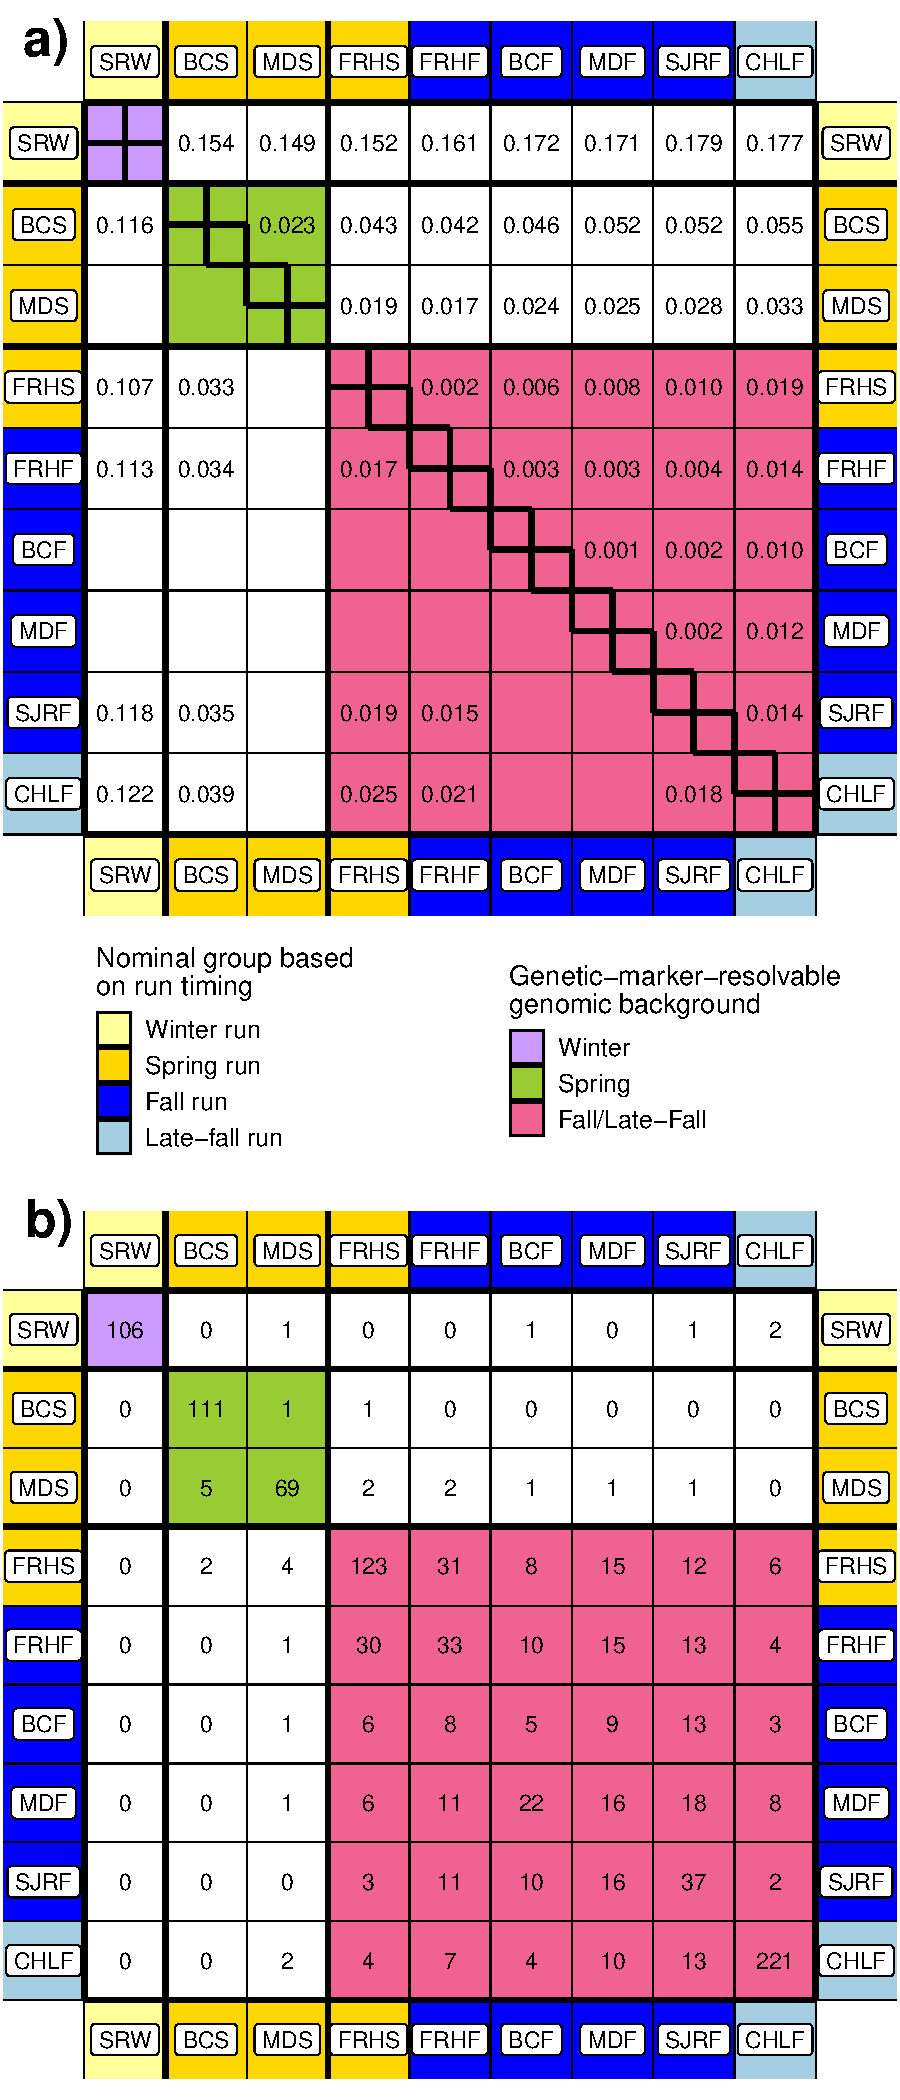
\includegraphics[width=0.35\textwidth]{images/assign_and_fst_table.pdf}
\end{center}
\caption[\examplecap]{\examplecap}
\label{fig:example}
\end{figure*}
